\section{Faster R-CNN}
\begin{frame}[allowframebreaks]
    \frametitle{\textsc{目录}} \vspace{-0.3cm}
    \begin{spacing}{0.0}
        \tableofcontents[currentsection,hideallsubsections]
    \end{spacing}   % 若不想要目录, 注释掉该句
\end{frame}

\begin{frame}
    \vspace{0.5em}
    \noindent\large\textbf{Faster R-CNN}\\
    \vspace{0.5em}
    Faster R-CNN是一个较为成熟的二阶段Anchor-based目标检测算法\\
    \vspace{0.5em}
    \begin{figure}
        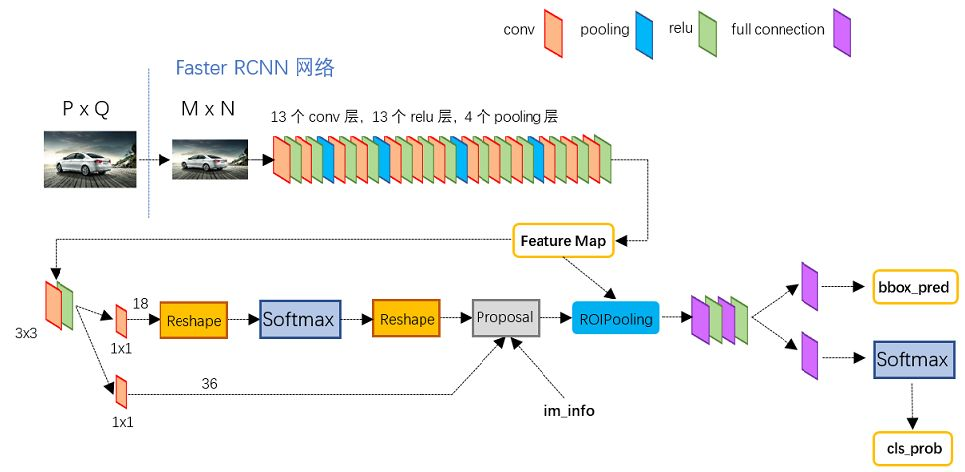
\includegraphics[width=\linewidth]{fasterrcnn.jpg}
    \end{figure}
\end{frame}

\begin{frame}[allowframebreaks]
    \vspace{-0.2cm}
    {\noindent\large\textbf{实现要点}}
    \vspace{0.4cm}
    \begin{itemize}
        \item[$ \bullet $] 锚框平铺
        \item[$ \bullet $] 边框回归,计算与变换
        \item[$ \bullet $] Proposal 筛选预测框
        \item[$ \bullet $] ROI Pooling 特征图采样
        \item[$ \bullet $] 训练过程
        \item[$ \bullet $] 数据处理
    \end{itemize}

\end{frame}

\begin{frame}
    \vspace{0.5em}
    \noindent\large\textbf{预设锚框}\\
    \vspace{0.5em}
    Faster R-CNN中设置了3种比例的锚框,1:1,1:2,2:1. 并且使用了多种尺寸,$64^2,128^2,256^2,512^2\cdots$\\
    \begin{figure}

        \subfloat{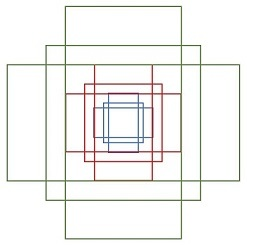
\includegraphics[width=0.3\linewidth]{anchors.jpg}}
        \hspace{0.4cm}
        \subfloat{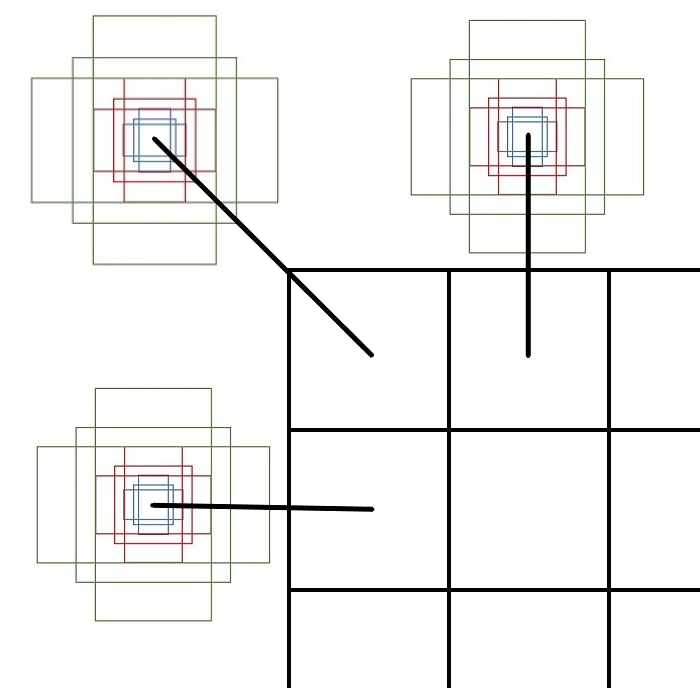
\includegraphics[width=0.3\linewidth]{anchorsposition.png}}
        \hspace{0.4cm}
        \subfloat{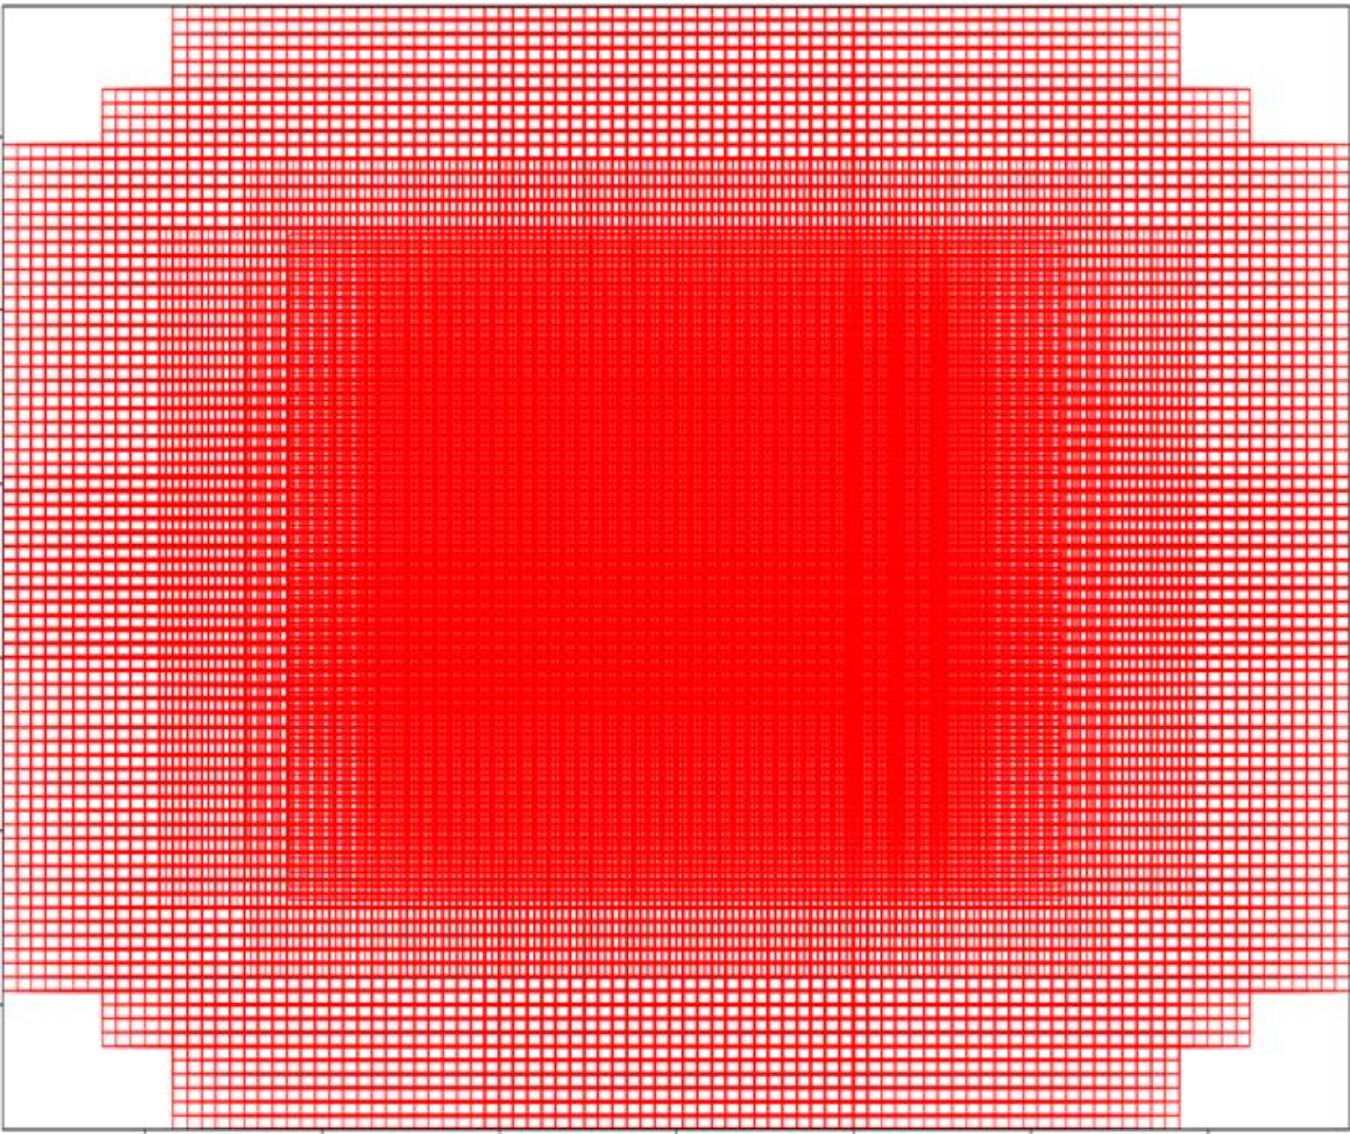
\includegraphics[width=0.3\linewidth]{uTools_1650882249335.png}}
    \end{figure}
    \vspace{0.5em}
    \noindent\large\textbf{锚框平铺}\\
    \vspace{0.5em}
    将图片分割为$P\times Q$的网格,在每一个网格上应用预设锚框,则锚框数量一共有$3\times P\times Q\times S$,其中$S$为应用的尺寸的数量.
\end{frame}
% \begin{frame}
%     \large
%     \textcolor{vscodedef}{def}  \textcolor{vscodefuncation}{tileAnchors}\textcolor{vscodebracket}{(}\\
%     \qquad\textcolor{vscodeparameter}{anchors}:\textcolor{vscodeclass}{Tensor},\\
%     \qquad\textcolor{vscodeparameter}{gridsize}:\textcolor{vscodeclass}{Tuple}\textcolor{vscodecomment}{[}\textcolor{vscodeclass}{int},\textcolor{vscodeclass}{int}\textcolor{vscodecomment}{]},\\
%     \qquad\textcolor{vscodeparameter}{imagesize}:\textcolor{vscodeclass}{Tuple}\textcolor{vscodecomment}{[}\textcolor{vscodeclass}{int},\textcolor{vscodeclass}{int}\textcolor{vscodecomment}{]}\\
%     \qquad\textcolor{vscodebracket}{)}->\textcolor{vscodeclass}{Tensor}:\\
%     \vspace{0.2em}
%     \qquad\textcolor{vscodeparameter}{baselength}=\textcolor{vscodeclass}{Tensor}\textcolor{vscodebracket}{(}\textcolor{vscodeparameter}{imagesize}\textcolor{vscodebracket}{)}/\textcolor{vscodeclass}{Tensor}\textcolor{vscodebracket}{(}\textcolor{vscodeparameter}{gridsize}\textcolor{vscodebracket}{)}\\
%     \vspace{0.2em}
%     \qquad\textcolor{vscodeparameter}{basepos}=\textcolor{vscodeclass}{torch}.\textcolor{vscodefuncation}{stack}\textcolor{vscodebracket}{(}\textcolor{vscodeclass}{torch}.\textcolor{vscodefuncation}{meshgrid}\textcolor{vscodecomment}{(}\\
%     \qquad\qquad\textcolor{vscodeclass}{torch}.\textcolor{vscodefuncation}{arange}\textcolor{vscode3bracket}{(}\textcolor{vscodeparameter}{baselength}\textcolor{vscodebracket}{[}\textcolor{vscodecomment}{0}\textcolor{vscodebracket}{]}/\textcolor{vscodecomment}{2},\textcolor{vscodeparameter}{imagesize}\textcolor{vscodebracket}{[}\textcolor{vscodecomment}{0}\textcolor{vscodebracket}{]},\textcolor{vscodeparameter}{baselength}\textcolor{vscodebracket}{[}\textcolor{vscodecomment}{1}\textcolor{vscodebracket}{]}\textcolor{vscodebracket}{)},\\
%     \qquad\qquad\textcolor{vscodeclass}{torch}.\textcolor{vscodefuncation}{arange}\textcolor{vscode3bracket}{(}\textcolor{vscodeparameter}{baselength}\textcolor{vscodebracket}{[}\textcolor{vscodecomment}{1}\textcolor{vscodebracket}{]}/\textcolor{vscodecomment}{2},\textcolor{vscodeparameter}{imagesize}\textcolor{vscodebracket}{[}\textcolor{vscodecomment}{1}\textcolor{vscodebracket}{]},\textcolor{vscodeparameter}{baselength}\textcolor{vscodebracket}{[}\textcolor{vscodecomment}{1}\textcolor{vscodebracket}{]}\textcolor{vscodebracket}{)},\\
%     \qquad\qquad\textcolor{vscodeparameter}{indexing}=\textcolor{vscode3bracket}{'xy'}\textcolor{vscodecomment}{)},\textcolor{vscodeparameter}{dim}=-\textcolor{vscodecomment}{1}\textcolor{vscodebracket}{)}  \textcolor{vscodecomment}{\# (H,W,2)}\\
%     \vspace{0.2em}
%     \qquad\textcolor{vscodeparameter}{baseanc}=\textcolor{vscodeclass}{torch}.\textcolor{vscodefuncation}{zeros}\textcolor{vscodebracket}{(}\textcolor{vscodecomment}{(}*\textcolor{vscodeparameter}{basepos}.\textcolor{vscodeparameter}{shape}\textcolor{vscode3bracket}{[}:\textcolor{vscodecomment}{2}\textcolor{vscode3bracket}{]},\textcolor{vscodeparameter}{anchors}.\textcolor{vscodeparameter}{shape}\textcolor{vscode3bracket}{[}\textcolor{vscodecomment}{0}\textcolor{vscode3bracket}{]},\textcolor{vscodecomment}{4}\textcolor{vscodecomment}{)}\textcolor{vscodebracket}{)}\\
%     \vspace{0.2em}
%     \qquad\textcolor{vscodeparameter}{baseanc}\textcolor{vscodebracket}{[}...,:\textcolor{vscodecomment}{2}\textcolor{vscodebracket}{]}=\textcolor{vscodeparameter}{basepos}.\textcolor{vscodefuncation}{unsqueeze}\textcolor{vscodebracket}{(}-\textcolor{vscodecomment}{2}\textcolor{vscodebracket}{)}-\textcolor{vscodeparameter}{anchors}/\textcolor{vscodecomment}{2}\\
%     \vspace{0.2em}
%     \qquad\textcolor{vscodeparameter}{baseanc}\textcolor{vscodebracket}{[}...,\textcolor{vscodecomment}{2}:\textcolor{vscodebracket}{]}=\textcolor{vscodeparameter}{basepos}.\textcolor{vscodefuncation}{unsqueeze}\textcolor{vscodebracket}{(}-\textcolor{vscodecomment}{2}\textcolor{vscodebracket}{)}+\textcolor{vscodeparameter}{anchors}/\textcolor{vscodecomment}{2}\\
%     \vspace{0.2em}
%     \qquad\textcolor{vscodereturn}{return} \textcolor{vscodeparameter}{baseanc}
% \end{frame}

\begin{frame}
    \vspace{0.5em}
    \noindent\large\textbf{边框回归}\\
    \vspace{0.5em}
    在将锚框平铺到整张图像后,预设锚框基本上覆盖了所有目标,但是还不够精确,而边框回归让预测框更加准确.Faster R-CNN使用了如下形式的变换将锚框$A$映射到预测框$G$:
    \vspace{1.5em}
    \begin{flalign*}
        G_x & =A_wd_x(A)+A_x    \\
        G_y & =A_gd_y(A)+A_y    \\
        G_w & =A_wexp(d_w(A))   \\
        G_h & =A_hexp(d_h(A)) &
    \end{flalign*}
    \vspace{-4cm}
    \begin{figure}
        \hspace{4.7cm}
        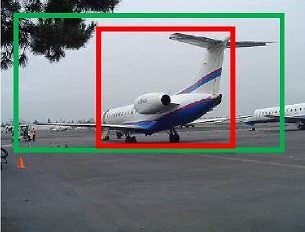
\includegraphics[width=0.4\linewidth]{reg.jpg}
    \end{figure}
    因此对预测框的校准问题就变成了对$d_x(A) d_y(A) d_w(A) d_y(A)$的回归问题

\end{frame}

% \begin{frame}
%     \large
%     \textcolor{vscodedef}{def}  \textcolor{vscodefuncation}{calculatedxywh}\textcolor{vscodebracket}{(}\textcolor{vscodeparameter}{anchors}:\textcolor{vscodeclass}{Tensor},\textcolor{vscodeparameter}{boxes}:\textcolor{vscodeclass}{Tensor}\textcolor{vscodebracket}{)}->\textcolor{vscodeclass}{Tensor}:\\
%     \vspace{0.2em}
%     \qquad\textcolor{vscodecomment}{\# anchors:(...,4) boxes:(...,4)}\\

%     \qquad\textcolor{vscodeparameter}{dxywh}=\textcolor{vscodeclass}{torch}.\textcolor{vscodefuncation}{zeros\_like}\textcolor{vscodebracket}{(}\textcolor{vscodeparameter}{anchors}\textcolor{vscodebracket}{)}\\

%     \qquad\textcolor{vscodeparameter}{dxywh}\textcolor{vscodebracket}{[}...,:\textcolor{vscodecomment}{2}\textcolor{vscodebracket}{]}=\textcolor{vscodebracket}{(}\textcolor{vscodeparameter}{boxes}\textcolor{vscodecomment}{[}...,:\textcolor{vscodecomment}{2]}-\textcolor{vscodecomment}{anchors}\textcolor{vscodecomment}{[}...,:\textcolor{vscodecomment}{2]}\textcolor{vscodebracket}{)}/\textcolor{vscodeparameter}{anchors}\textcolor{vscodebracket}{[}...,\textcolor{vscodecomment}{2}:\textcolor{vscodebracket}{]}\\

%     \qquad\textcolor{vscodeparameter}{dxywh}\textcolor{vscodebracket}{[}...,\textcolor{vscodecomment}{2}:\textcolor{vscodebracket}{]}=\textcolor{vscodeclass}{torch}.\textcolor{vscodefuncation}{log}\textcolor{vscodebracket}{(}\textcolor{vscodeparameter}{boxes}\textcolor{vscodecomment}{[}...,\textcolor{vscodecomment}{2}:\textcolor{vscodecomment}{]}/\textcolor{vscodeparameter}{anchors}\textcolor{vscodecomment}{[}...,\textcolor{vscodecomment}{2}:\textcolor{vscodecomment}{]}\textcolor{vscodebracket}{)}\\

%     \qquad\textcolor{vscodeparameter}{dxywh}=\textcolor{vscodeparameter}{dxywh}.\textcolor{vscodefuncation}{nan\_to\_num}\textcolor{vscodebracket}{(}\textcolor{vscodecomment}{0}\textcolor{vscodebracket}{)}

%     \qquad\textcolor{vscodereturn}{return} \textcolor{vscodeparameter}{dxywh}

%     \vspace{0.5em}

%     \textcolor{vscodedef}{def}  \textcolor{vscodefuncation}{applydxywh}\textcolor{vscodebracket}{(}\textcolor{vscodeparameter}{anchors}:\textcolor{vscodeclass}{Tensor},\textcolor{vscodeparameter}{dxywh}:\textcolor{vscodeclass}{Tensor}\textcolor{vscodebracket}{)}->\textcolor{vscodeclass}{Tensor}:\\

%     \qquad\textcolor{vscodecomment}{\# anchors:(...,4) dxywh:(...,4)}\\

%     \qquad\textcolor{vscodeparameter}{matrix}=\textcolor{vscodeclass}{torch}.\textcolor{vscodefuncation}{zeros}\textcolor{vscodebracket}{(}*\textcolor{vscodeparameter}{dxywh}.\textcolor{vscodeparameter}{shape},\textcolor{vscodecomment}{4}\textcolor{vscodebracket}{)}

%     \qquad\textcolor{vscodeparameter}{matrix}\textcolor{vscodebracket}{[}...,:\textcolor{vscodecomment}{2},\textcolor{vscodecomment}{2}:\textcolor{vscodebracket}{]}=\textcolor{vscodeparameter}{dxywh}\textcolor{vscodebracket}{[}...,:\textcolor{vscodecomment}{2}\textcolor{vscodebracket}{]}.\textcolor{vscodefuncation}{diag\_embed}\textcolor{vscodebracket}{()}\\

%     \qquad\textcolor{vscodeparameter}{matrix}\textcolor{vscodebracket}{[}...,:\textcolor{vscodecomment}{2},:\textcolor{vscodecomment}{2}\textcolor{vscodebracket}{]}=\textcolor{vscodecomment}{1}-\textcolor{vscodeparameter}{matrix}\textcolor{vscodebracket}{[}...,:\textcolor{vscodecomment}{2},\textcolor{vscodecomment}{2}:\textcolor{vscodebracket}{]}\\

%     \qquad\textcolor{vscodeparameter}{matrix}\textcolor{vscodebracket}{[}...,\textcolor{vscodecomment}{2}:,\textcolor{vscodecomment}{2}:\textcolor{vscodebracket}{]}=\textcolor{vscodeclass}{torch}.\textcolor{vscodefuncation}{exp}\textcolor{vscodebracket}{(}\textcolor{vscodeparameter}{dxywh}\textcolor{vscodecomment}{[}...,\textcolor{vscodecomment}{2}:\textcolor{vscodebracket}{]}\textcolor{vscodebracket}{)}.\textcolor{vscodefuncation}{diag\_embed}\textcolor{vscodebracket}{()}\\

%     \qquad\textcolor{vscodeparameter}{matrix}\textcolor{vscodebracket}{[}...,\textcolor{vscodecomment}{2}:,:\textcolor{vscodecomment}{2}\textcolor{vscodebracket}{]}=\textcolor{vscodecomment}{1}-\textcolor{vscodeparameter}{matrix}\textcolor{vscodebracket}{[}...,\textcolor{vscodecomment}{2}:,\textcolor{vscodecomment}{2}:\textcolor{vscodebracket}{]}\\

%     \qquad\textcolor{vscodeparameter}{anchors}=\textcolor{vscodebracket}{(}\textcolor{vscodeparameter}{matrix}@\textcolor{vscodeparameter}{anchors}.\textcolor{vscodefuncation}{unsqueeze}\textcolor{vscodecomment}{(}-\textcolor{vscodecomment}{1)}\textcolor{vscodebracket}{)}.\textcolor{vscodefuncation}{squeeze}\textcolor{vscodebracket}{(}-\textcolor{vscodecomment}{1}\textcolor{vscodebracket}{)}\\

%     \qquad\textcolor{vscodereturn}{return} \textcolor{vscodeparameter}{anchors}
% \end{frame}

\begin{frame}
    \vspace{0.5em}
    \noindent\large\textbf{RPN层}\\
    \vspace{0.5em}
    RPN 层的主要工作是预测预设框内是否有目标物体以及预测从预设框到预测框的变换$d_{xywh}$
    \begin{figure}
        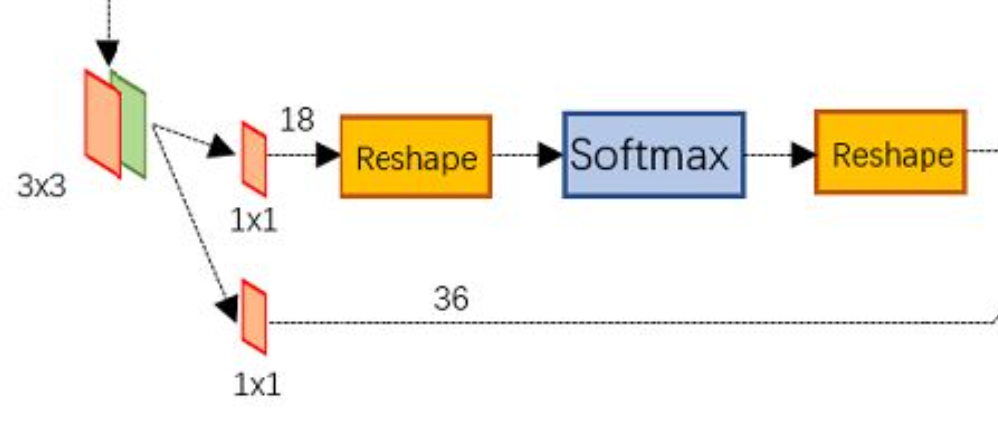
\includegraphics[width=0.8\linewidth]{RPNlayer.png}
    \end{figure}
    其中预设框内是否有目标物体是一个二分类问题,使用通道为$2K$的$1\times 1$卷积实现并且在reshape后经过Softmax运算,预测变换使用的是通道为$4K$的$1\times 1$卷积


\end{frame}

\begin{frame}
    \vspace{0.5em}
    \noindent\large\textbf{Proposal层}\\
    \vspace{0.5em}
    Proposal Layer的工作是根据RPN层的预测信息挑选出合适的预测框,算法如下:\\
    \vspace{0.2em}
    输入:预设框内有物体的置信度,预设框,变换的回归估计
    \vspace{0.2em}
    \begin{itemize}
        \item[1]根据置信度从大到小排序,选出置信度最高的N个预测框
        \item[2]使用变换的回归估计对预设框进行修正
        \item[3]修正超出图像边界的预测框
        \item[4]剔除过小的预测框
        \item[5]对剩余预测框执行非极大值抑制(NMS)
    \end{itemize}
    \vspace{0.5em}
    到这一步已经完成了"在哪里"和"有哪些"的任务,后面的工作就是分类以及对结果的轻微修正
\end{frame}

% \begin{frame}
%     \large
%     \textcolor{vscodedef}{def}  \textcolor{vscodefuncation}{proposal}\textcolor{vscodebracket}{(}\textcolor{vscodeparameter}{anchs}:\textcolor{vscodeclass}{Tensor},\textcolor{vscodeparameter}{boxreg}:\textcolor{vscodeclass}{Tensor},\textcolor{vscodeparameter}{score}:\textcolor{vscodeclass}{Tensor},\textcolor{vscodeparameter}{N}:\textcolor{vscodeclass}{int},\\
%     \qquad\textcolor{vscodeparameter}{imagesize}:\textcolor{vscodeclass}{Tuple}\textcolor{vscodecomment}{[}\textcolor{vscodeclass}{int},\textcolor{vscodeclass}{int}\textcolor{vscodecomment}{]},\textcolor{vscodeparameter}{minsize}:\textcolor{vscodeclass}{int},\textcolor{vscodeparameter}{threshold}:\textcolor{vscodeclass}{float}\textcolor{vscodebracket}{)}->\textcolor{vscodeclass}{Tensor}:\\

%     \qquad\textcolor{vscodecomment}{\# anchors:(N,H,W,K,4) boxreg:(N,H,W,K,4) score:{N,H,W,K}}\\

%     \qquad\textcolor{vscodeparameter}{idx}=\textcolor{vscodeparameter}{score}>\textcolor{vscodecomment}{0.5}\\

%     \qquad\textcolor{vscodeparameter}{anchs},\textcolor{vscodeparameter}{boxreg},\textcolor{vscodeparameter}{score}=\textcolor{vscodefuncation}{applyIndex}\textcolor{vscodebracket}{(}\textcolor{vscodeparameter}{idx},\textcolor{vscodeparameter}{anchs},\textcolor{vscodeparameter}{boxreg},\textcolor{vscodeparameter}{score}\textcolor{vscodebracket}{)}\\

%     \qquad\textcolor{vscodereturn}{if} \textcolor{vscodeparameter}{score}.\textcolor{vscodeparameter}{shape}\textcolor{vscodebracket}{[}\textcolor{vscodecomment}{0}\textcolor{vscodebracket}{]}>\textcolor{vscodeparameter}{N}:\\

%     \qquad\qquad\textcolor{vscodeparameter}{idx}=\textcolor{vscodeparameter}{score}.\textcolor{vscodefuncation}{topk}\textcolor{vscodebracket}{(}\textcolor{vscodeparameter}{N}\textcolor{vscodebracket}{)}.\textcolor{vscodeparameter}{indices}\\

%     \qquad\qquad\textcolor{vscodeparameter}{anchs},\textcolor{vscodeparameter}{boxreg},\textcolor{vscodeparameter}{score}=\textcolor{vscodefuncation}{applyIndex}\textcolor{vscodebracket}{(}\textcolor{vscodeparameter}{idx},\textcolor{vscodeparameter}{anchs},\textcolor{vscodeparameter}{boxreg},\textcolor{vscodeparameter}{score}\textcolor{vscodebracket}{)}

%     \qquad\textcolor{vscodeparameter}{boxes}=\textcolor{vscodefuncation}{applydxywh}\textcolor{vscodebracket}{(}\textcolor{vscodeparameter}{anchors},\textcolor{vscodeparameter}{boxreg}\textcolor{vscodebracket}{)}\\

%     \qquad\textcolor{vscodeparameter}{boxes}=\textcolor{vscodefuncation}{clip\_boxes\_to\_image}\textcolor{vscodebracket}{(}\textcolor{vscodeparameter}{boxes},\textcolor{vscodeparameter}{imagesize}\textcolor{vscodebracket}{)}\\

%     \qquad\textcolor{vscodeparameter}{idx}=\textcolor{vscodefuncation}{remove\_small\_boxes}\textcolor{vscodebracket}{(}\textcolor{vscodeparameter}{boxes},\textcolor{vscodeparameter}{minsize}\textcolor{vscodebracket}{)}\\

%     \qquad\textcolor{vscodeparameter}{boxes},\textcolor{vscodeparameter}{score}=\textcolor{vscodefuncation}{applyIndex}\textcolor{vscodebracket}{(}\textcolor{vscodeparameter}{idx},\textcolor{vscodeparameter}{boxes},\textcolor{vscodeparameter}{score}\textcolor{vscodebracket}{)}\\

%     \qquad\textcolor{vscodeparameter}{idx}=\textcolor{vscodefuncation}{nms}\textcolor{vscodebracket}{(}\textcolor{vscodeparameter}{boxes},\textcolor{vscodeparameter}{minsize},\textcolor{vscodeparameter}{threshold}\textcolor{vscodebracket}{)}\\

%     \qquad\textcolor{vscodereturn}{return} \textcolor{vscodeparameter}{boxes}\textcolor{vscodebracket}{[}\textcolor{vscodeparameter}{idx}\textcolor{vscodebracket}{]}.\textcolor{vscodefuncation}{clone}\textcolor{vscodebracket}{(}\textcolor{vscodebracket}{)}
% \end{frame}

\begin{frame}
    \vspace{0.5em}
    \noindent\large\textbf{ROI Pooling}\\
    \vspace{0.5em}
    Region of interest pooling是对选定的区域进行采样的过程,在得到预测框后需要将区域的图像输入CNN分类器当中,这要求这些区域的分辨率保持一致.\\
    \vspace{0.2em}
    首先,Faster R-CNN是在下采样后的特征图上进行采样的,因此需要把预测框转换为特征图的尺寸.\\
    \vspace{0.2em}
    接下来,对预测框进行取整来对特征图进行切片并将进行池化,使特征图切片的大小统一.这里使用自适应最大/平均池化来代替原论文的复杂池化过程.
    \begin{figure}
        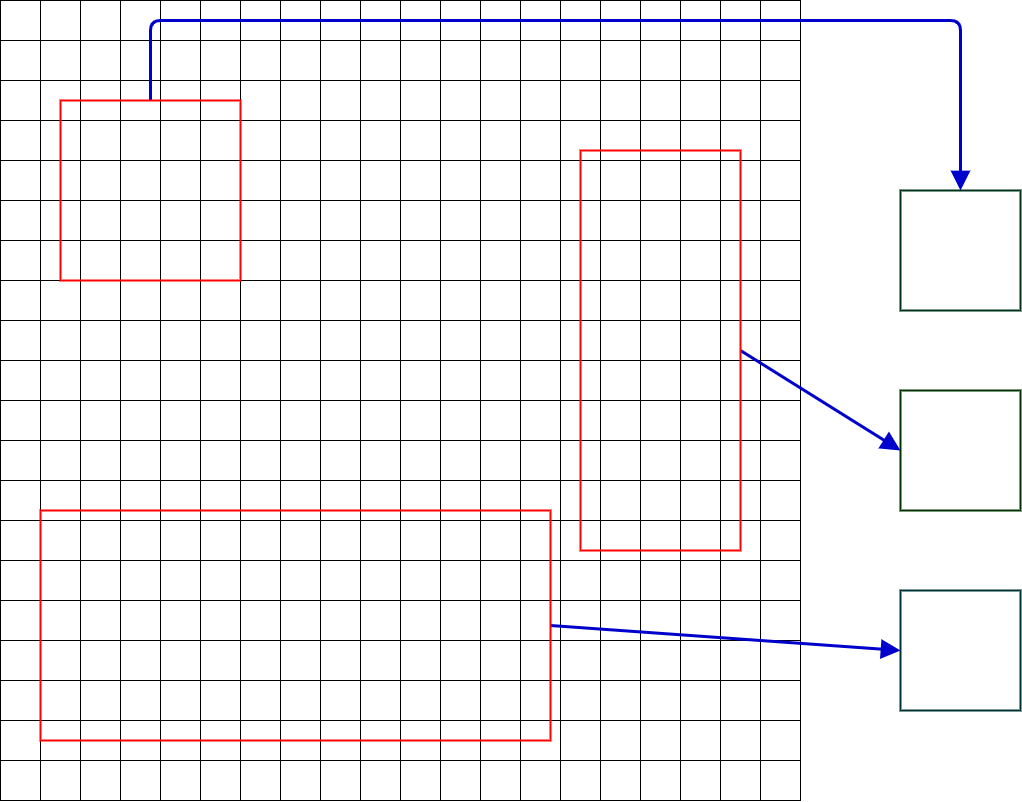
\includegraphics[width=0.4\linewidth]{roipooling.png}
    \end{figure}
\end{frame}


% \begin{frame}
%     \large
%     \textcolor{vscodedef}{def}  \textcolor{vscodefuncation}{roiPooling}\textcolor{vscodebracket}{(}\\
%     \qquad\textcolor{vscodeparameter}{feamap}:\textcolor{vscodeclass}{Tensor},\\
%     \qquad\textcolor{vscodeparameter}{boxes}:\textcolor{vscodeclass}{Tensor},\\
%     \qquad\textcolor{vscodeparameter}{imgsize}:\textcolor{vscodeclass}{Tuple}\textcolor{vscodecomment}{[}\textcolor{vscodeclass}{int},\textcolor{vscodeclass}{int}\textcolor{vscodecomment}{]},\\
%     \qquad\textcolor{vscodeparameter}{outsize}:\textcolor{vscodeclass}{Tuple}\textcolor{vscodecomment}{[}\textcolor{vscodeclass}{int},\textcolor{vscodeclass}{int}\textcolor{vscodecomment}{]}\textcolor{vscodebracket}{)}:\\

%     \qquad\textcolor{vscodecomment}{\# feamap (1,C,H,W) boxes:(N,4)}\\

%     \qquad\textcolor{vscodeparameter}{h},\textcolor{vscodeparameter}{w}=\textcolor{vscodeparameter}{feamap}.\textcolor{vscodeparameter}{shape}\textcolor{vscodebracket}{[}-\textcolor{vscodecomment}{2}:\textcolor{vscodebracket}{]}\\

%     \qquad\textcolor{vscodeparameter}{boxes}=\textcolor{vscodefuncation}{resizeBox}\textcolor{vscodebracket}{(}\textcolor{vscodeparameter}{imgsize},\textcolor{vscodecomment}{(}\textcolor{vscodeparameter}{w},\textcolor{vscodeparameter}{h}\textcolor{vscodecomment}{)},\textcolor{vscodeparameter}{boxes}\textcolor{vscodebracket}{)}\\

%     \qquad\textcolor{vscodeparameter}{boxes}=\textcolor{vscodeparameter}{boxes}.\textcolor{vscodefuncation}{floor}\textcolor{vscodebracket}{()}\\

%     \qquad\textcolor{vscodeparameter}{roiarea}=\textcolor{vscodeclass}{torch}.\textcolor{vscodefuncation}{cat}\textcolor{vscodebracket}{(}\textcolor{vscodecomment}{[}\textcolor{vscodeclass}{F}.\textcolor{vscodefuncation}{adaptive\_avg\_pool2d}\textcolor{vscode3bracket}{(}\\
%     \qquad\qquad\textcolor{vscodeparameter}{feamap}\textcolor{vscodebracket}{[}...,\textcolor{vscodeparameter}{box}\textcolor{vscodecomment}{[1]}:\textcolor{vscodeparameter}{box}\textcolor{vscodecomment}{[3]},\textcolor{vscodeparameter}{box}\textcolor{vscodecomment}{[0]}:\textcolor{vscodeparameter}{box}\textcolor{vscodecomment}{[2]}\textcolor{vscodebracket}{]},\textcolor{vscodeparameter}{outsize}\textcolor{vscode3bracket}{)}\\
%     \qquad\qquad\textcolor{vscodereturn}{for} \textcolor{vscodeparameter}{box} \textcolor{vscodereturn}{in} \textcolor{vscodeparameter}{boxes}\textcolor{vscodecomment}{]}\textcolor{vscodebracket}{)}\

%     \qquad\textcolor{vscodereturn}{return} \textcolor{vscodeparameter}{roiarea}



% \end{frame}

\begin{frame}
    \vspace{0.5em}
    \noindent\large\textbf{第二阶段}\\
    \vspace{0.5em}
    第二阶段的任务是一个简单的分类+回归任务.
    \begin{itemize}
        \item[$ \bullet $]输 入:ROI区域特征图([M,C,H,W])
        \item[$ \bullet $]网 络:卷积网络
        \item[$ \bullet $]输出1:基于第一次预测框的更精确的预测框回归
        \item[$ \bullet $]输出2:ROI区域物体类别
    \end{itemize}
    \begin{figure}
        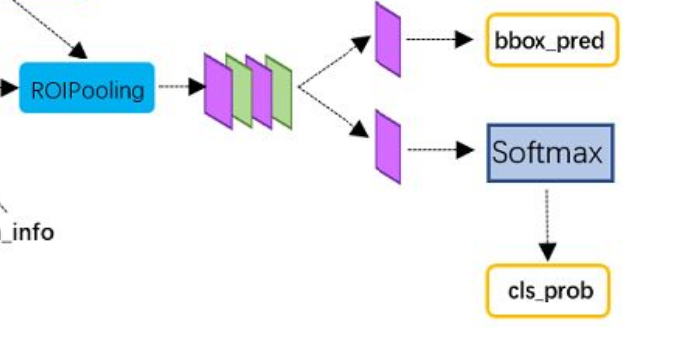
\includegraphics[width=0.6\linewidth]{uTools_1651760901375.png}
    \end{figure}
\end{frame}

\begin{frame}
    \vspace{0.5em}
    \noindent\large\textbf{训练过程}\\
    \vspace{0.5em}
    Faster R-CNN的特征提取器使用预训练的卷积网络(resnet18、vgg16等)
    \begin{itemize}
        \item[1]固定特征提取器,训练RPN层
        \item[2]固定特征提取器和RPN,训练分割部分
        \item[3]整体训练
    \end{itemize}
    在两个阶段的训练当中都有回归任务和分类任务,回归任务使用的是L1 Smooth Loss,分类使用CrossEntrpyLoss
    $$
        l = \begin{cases}
            0.5 (y - \hat{y})^2 / \beta, & \text{if } |y - \hat{y}| < \beta \\
            |y - \hat{y}| - 0.5 \beta,   & \text{otherwise }
        \end{cases}
    $$


\end{frame}

\begin{frame}
    \vspace{0.5em}
    \noindent\large\textbf{数据处理}\\
    \vspace{0.5em}
    在实际训练时,需要将原始数据格式转换成模型需要的输入或标签,这里以COCO数据集为例说明需要做哪些处理:
    \begin{itemize}
        \item[1]获取图片、定位框、目标分类标签
        \item[2]将图片resize到指定大小方便训练
        \item[3]将定位框转换到新的坐标系
        \item[4]生成预设框内有/无物体的分类标签
        \item[5]生成预设框到定位框的变换dxywh
    \end{itemize}
    其中生成的两种数据仅训练RPN层时使用,定位框与分类标签在训练第二阶段网络时使用.
\end{frame}

% \begin{frame}
%     \textcolor{vscodedef}{class}  \textcolor{vscodeclass}{FasterRCNNCOCODataset}\textcolor{vscodebracket}{(}\textcolor{vscodeclass}{CocoDetection}\textcolor{vscodebracket}{)}:\\

%     \qquad\textcolor{vscodedef}{def} \textcolor{vscodefuncation}{\_\_init\_\_}\textcolor{vscodebracket}{(}\textcolor{vscodeparameter}{self},\\
%     \qquad\qquad\textcolor{vscodeparameter}{root}:\textcolor{vscodeclass}{str},\\
%     \qquad\qquad\textcolor{vscodeparameter}{annFile}:\textcolor{vscodeclass}{str},\\
%     \qquad\qquad\textcolor{vscodeparameter}{gridsize}:\textcolor{vscodeclass}{Tuple}\textcolor{vscodecomment}{[}\textcolor{vscodeclass}{int},\textcolor{vscodeclass}{int}\textcolor{vscodecomment}{]},\\
%     \qquad\qquad\textcolor{vscodeparameter}{imagesize}:\textcolor{vscodeclass}{Tuple}\textcolor{vscodecomment}{[}\textcolor{vscodeclass}{int},\textcolor{vscodeclass}{int}\textcolor{vscodecomment}{]},\\
%     \qquad\qquad\textcolor{vscodeparameter}{imagetransformers}:\textcolor{vscodeclass}{Optional}\textcolor{vscodecomment}{[}\textcolor{vscodeclass}{Callable}\textcolor{vscodecomment}{]},\\
%     \qquad\qquad\textcolor{vscodeparameter}{outputItems}:\textcolor{vscodeclass}{List}\textcolor{vscodecomment}{[}\textcolor{vscodeclass}{str}\textcolor{vscodecomment}{]}\textcolor{vscodebracket}{)}:\\

%     \qquad\qquad\textcolor{vscodeclass}{super}\textcolor{vscodebracket}{()}.\textcolor{vscodefuncation}{\_\_init\_\_}\textcolor{vscodebracket}{(}\textcolor{vscodeparameter}{root},\textcolor{vscodeparameter}{annFile}\textcolor{vscodebracket}{)}\\

%     \qquad\qquad\textcolor{vscodeparameter}{self}.\textcolor{vscodeparameter}{anchorsWH}=\textcolor{vscodeparameter}{anchors}

%     \qquad\qquad\textcolor{vscodeparameter}{self}.\textcolor{vscodeparameter}{anchors}=\textcolor{vscodefuncation}{tileAnchors}\textcolor{vscodebracket}{(}\textcolor{vscodeparameter}{anchors},\textcolor{vscodeparameter}{anchors}

%     \qquad\textcolor{vscodedef}{def}  \textcolor{vscodefuncation}{getPositiveNegativeRegression}\textcolor{vscodebracket}{(}\textcolor{vscodeparameter}{self},\textcolor{vscodeparameter}{boxes}:\textcolor{vscodeclass}{Tensor}\textcolor{vscodebracket}{)}:\\

%     \qquad\qquad\textcolor{vscodeparameter}{ious}=\textcolor{vscodefuncation}{boxIou}\textcolor{vscodebracket}{(}\textcolor{vscodeparameter}{self}.\textcolor{vscodeparameter}{anchors}.\textcolor{vscodefuncation}{view}\textcolor{vscodecomment}{(}-\textcolor{vscodecomment}{1},\textcolor{vscodecomment}{4}\textcolor{vscodecomment}{)},\\
%     \qquad\qquad\qquad\textcolor{vscodefuncation}{box\_convert}\textcolor{vscodecomment}{(}\textcolor{vscodeparameter}{boxes},\textcolor{vscode3bracket}{'xywh'},\textcolor{vscode3bracket}{'xyxy'}\textcolor{vscodecomment}{)}\textcolor{vscodebracket}{)}\\

%     \qquad\qquad\textcolor{vscodeparameter}{ious}=\textcolor{vscodeparameter}{ious}.\textcolor{vscodefuncation}{reshape}\textcolor{vscodebracket}{(}*\textcolor{vscodeparameter}{self}.\textcolor{vscodeparameter}{anchors}.\textcolor{vscodeparameter}{shape}\textcolor{vscodecomment}{[}:\textcolor{vscodecomment}{3]},\textcolor{vscodeparameter}{boxes}.\textcolor{vscodeparameter}{shape}\textcolor{vscodecomment}{[0]}\textcolor{vscodebracket}{)}\\

%     \qquad\qquad\textcolor{vscodeparameter}{maxiou},\textcolor{vscodeparameter}{indexes}=\textcolor{vscodeparameter}{ious}.\textcolor{vscodefuncation}{max}\textcolor{vscodebracket}{(}-\textcolor{vscodecomment}{1}\textcolor{vscodebracket}{)}\\

%     \qquad\qquad\textcolor{vscodeparameter}{currentgt}=\textcolor{vscodeparameter}{boxes}\textcolor{vscodebracket}{[}\textcolor{vscodeparameter}{indexes}\textcolor{vscodebracket}{]}\\

%     \qquad\textcolor{vscodereturn}{return} \textcolor{vscodeclass}{torch}.\textcolor{vscodefuncation}{stack}\textcolor{vscodebracket}{(}\textcolor{vscodecomment}{[}\textcolor{vscode3bracket}{(}\textcolor{vscodeparameter}{maxiou}>\textcolor{vscodecomment}{0.7}\textcolor{vscode3bracket}{)}.\textcolor{vscodefuncation}{long}\textcolor{vscode3bracket}{()},\textcolor{vscode3bracket}{(}\textcolor{vscodeparameter}{maxiou}<\textcolor{vscodecomment}{0.3}\textcolor{vscode3bracket}{)}.\textcolor{vscodefuncation}{long}\textcolor{vscode3bracket}{()}\textcolor{vscodecomment}{]}\textcolor{vscodebracket}{)},\\
%     \qquad\qquad\qquad\textcolor{vscodefuncation}{calculatedxywh}\textcolor{vscodebracket}{(}\textcolor{vscodeparameter}{self}.\textcolor{vscodeparameter}{anchors},\textcolor{vscodeparameter}{currentgt}\textcolor{vscodebracket}{)}

% \end{frame}

% \begin{frame}
%     \qquad\textcolor{vscodedef}{def}  \textcolor{vscodefuncation}{\_\_getitem\_\_}\textcolor{vscodebracket}{(}\textcolor{vscodeparameter}{self},\textcolor{vscodeparameter}{index}:\textcolor{vscodeclass}{int}\textcolor{vscodebracket}{)}:\\

%     \qquad\qquad\textcolor{vscodeparameter}{image},\textcolor{vscodeparameter}{target}=\textcolor{vscodeclass}{super}\textcolor{vscodebracket}{()}.\textcolor{vscodefuncation}{\_\_getitem\_\_}\textcolor{vscodebracket}{()}\\

%     \qquad\qquad\textcolor{vscodeparameter}{image}=\textcolor{vscodeclass}{TF}.\textcolor{vscodefuncation}{to\_tensor}\textcolor{vscodebracket}{(}\textcolor{vscodeparameter}{image}\textcolor{vscodebracket}{)}\\

%     \qquad\qquad\textcolor{vscodeparameter}{h},\textcolor{vscodeparameter}{w}=\textcolor{vscodeparameter}{image}.\textcolor{vscodeparameter}{shape}\textcolor{vscodebracket}{[}-\textcolor{vscodecomment}{2}:\textcolor{vscodebracket}{]}\\

%     \qquad\qquad\textcolor{vscodeparameter}{image}=\textcolor{vscodeclass}{TF}.\textcolor{vscodefuncation}{resize}\textcolor{vscodebracket}{(}\textcolor{vscodeparameter}{image},\textcolor{vscodecomment}{(}\textcolor{vscodeparameter}{self}.\textcolor{vscodeparameter}{imagesize}\textcolor{vscode3bracket}{[}\textcolor{vscodecomment}{1}\textcolor{vscode3bracket}{]},\textcolor{vscodeparameter}{self}.\textcolor{vscodeparameter}{imagesize}\textcolor{vscode3bracket}{[}\textcolor{vscodecomment}{0}\textcolor{vscode3bracket}{]}\textcolor{vscodecomment}{)}\textcolor{vscodebracket}{)}\\

%     \qquad\qquad\textcolor{vscodereturn}{if} \textcolor{vscodeparameter}{self}.\textcolor{vscodeparameter}{imagetransformers}:

%     \qquad\qquad\qquad\textcolor{vscodeparameter}{image}=\textcolor{vscodeparameter}{self}.\textcolor{vscodeparameter}{imagetransformers}\textcolor{vscodebracket}{(}\textcolor{vscodeparameter}{image}\textcolor{vscodebracket}{)}\\

%     \qquad\qquad\textcolor{vscodeparameter}{bboxes}=\textcolor{vscodeclass}{Tensor}\textcolor{vscodebracket}{(}\textcolor{vscodecomment}{[}\textcolor{vscodeparameter}{\_}\textcolor{vscode3bracket}{['bbox']} \textcolor{vscodereturn}{for} \textcolor{vscodeparameter}{\_} \textcolor{vscodereturn}{in} \textcolor{vscodeparameter}{target}\textcolor{vscodecomment}{]}\textcolor{vscodebracket}{)}\\

%     \qquad\qquad\textcolor{vscodeparameter}{bboxes}=\textcolor{vscodefuncation}{resizeBox}\textcolor{vscodebracket}{(}\textcolor{vscodecomment}{(}\textcolor{vscodeparameter}{w},\textcolor{vscodeparameter}{h}\textcolor{vscodecomment}{)},\textcolor{vscodeparameter}{self}.\textcolor{vscodeparameter}{imagesize},\textcolor{vscodeparameter}{bboxes}\textcolor{vscodebracket}{)}\\

%     \qquad\qquad\textcolor{vscodeparameter}{category\_ids}=\textcolor{vscodeclass}{Tensor}\textcolor{vscodebracket}{(}\textcolor{vscodecomment}{[}\textcolor{vscodeparameter}{\_}\textcolor{vscode3bracket}{['category\_id']} \textcolor{vscodereturn}{for} \textcolor{vscodeparameter}{\_} \textcolor{vscodereturn}{in} \textcolor{vscodeparameter}{target}\textcolor{vscodecomment}{]}\textcolor{vscodebracket}{)}\\

%     \qquad\qquad\textcolor{vscodereturn}{if} \textcolor{vscode3bracket}{'positive\_negative'} \textcolor{vscodereturn}{in} \textcolor{vscodeparameter}{self}.\textcolor{vscodeparameter}{outputItems}:\\

%     \qquad\qquad\qquad\textcolor{vscodeparameter}{positive\_negative},\textcolor{vscodeparameter}{regression}=\\

%     \qquad\qquad\qquad\qquad\textcolor{vscodeparameter}{self}.\textcolor{vscodefuncation}{getPositiveNegativeRegression}\textcolor{vscodebracket}{(}\textcolor{vscodeparameter}{bboxes}\textcolor{vscodebracket}{)}\\

%     \qquad\qquad\textcolor{vscodeparameter}{result}=\textcolor{vscodebracket}{[]}\\

%     \qquad\qquad\textcolor{vscodereturn}{for} \textcolor{vscodeparameter}{\_} \textcolor{vscodereturn}{in} \textcolor{vscodeparameter}{self}.\textcolor{vscodeparameter}{outputItems}:\\

%     \qquad\qquad\qquad\textcolor{vscodeparameter}{result}.\textcolor{vscodefuncation}{append}\textcolor{vscodebracket}{(}\textcolor{vscodefuncation}{eval}\textcolor{vscodecomment}{(}\textcolor{vscodeparameter}{\_}\textcolor{vscodecomment}{)}\textcolor{vscodebracket}{)}\\

%     \qquad\qquad\textcolor{vscodereturn}{return} \textcolor{vscodeparameter}{result}
% \end{frame}
